% Options for packages loaded elsewhere
\PassOptionsToPackage{unicode}{hyperref}
\PassOptionsToPackage{hyphens}{url}
%
\documentclass[
]{article}
\usepackage{amsmath,amssymb}
\usepackage{lmodern}
\usepackage{iftex}
\ifPDFTeX
  \usepackage[T1]{fontenc}
  \usepackage[utf8]{inputenc}
  \usepackage{textcomp} % provide euro and other symbols
\else % if luatex or xetex
  \usepackage{unicode-math}
  \defaultfontfeatures{Scale=MatchLowercase}
  \defaultfontfeatures[\rmfamily]{Ligatures=TeX,Scale=1}
\fi
% Use upquote if available, for straight quotes in verbatim environments
\IfFileExists{upquote.sty}{\usepackage{upquote}}{}
\IfFileExists{microtype.sty}{% use microtype if available
  \usepackage[]{microtype}
  \UseMicrotypeSet[protrusion]{basicmath} % disable protrusion for tt fonts
}{}
\makeatletter
\@ifundefined{KOMAClassName}{% if non-KOMA class
  \IfFileExists{parskip.sty}{%
    \usepackage{parskip}
  }{% else
    \setlength{\parindent}{0pt}
    \setlength{\parskip}{6pt plus 2pt minus 1pt}}
}{% if KOMA class
  \KOMAoptions{parskip=half}}
\makeatother
\usepackage{xcolor}
\IfFileExists{xurl.sty}{\usepackage{xurl}}{} % add URL line breaks if available
\IfFileExists{bookmark.sty}{\usepackage{bookmark}}{\usepackage{hyperref}}
\hypersetup{
  pdftitle={Test2},
  pdfauthor={Paul Christmann},
  hidelinks,
  pdfcreator={LaTeX via pandoc}}
\urlstyle{same} % disable monospaced font for URLs
\usepackage[left=1.5cm,right=1.5cm,top=1.5cm,bottom=1.5cm]{geometry}
\usepackage{graphicx}
\makeatletter
\def\maxwidth{\ifdim\Gin@nat@width>\linewidth\linewidth\else\Gin@nat@width\fi}
\def\maxheight{\ifdim\Gin@nat@height>\textheight\textheight\else\Gin@nat@height\fi}
\makeatother
% Scale images if necessary, so that they will not overflow the page
% margins by default, and it is still possible to overwrite the defaults
% using explicit options in \includegraphics[width, height, ...]{}
\setkeys{Gin}{width=\maxwidth,height=\maxheight,keepaspectratio}
% Set default figure placement to htbp
\makeatletter
\def\fps@figure{htbp}
\makeatother
\setlength{\emergencystretch}{3em} % prevent overfull lines
\providecommand{\tightlist}{%
  \setlength{\itemsep}{0pt}\setlength{\parskip}{0pt}}
\setcounter{secnumdepth}{-\maxdimen} % remove section numbering
\usepackage[font={small,it}, labelfont={bf}]{caption}
\usepackage{amsmath}
\usepackage{booktabs}
\usepackage{caption}
\usepackage{longtable}
\ifLuaTeX
  \usepackage{selnolig}  % disable illegal ligatures
\fi

\title{Test2}
\author{Paul Christmann}
\date{2022-07-12}

\begin{document}
\maketitle

\hypertarget{the-expression-of-all-tras-associated-with-a-tissue-cannot-be-used-to-infer-organ-development}{%
\subsubsection{The expression of all TRAs associated with a tissue
cannot be used to infer organ
development}\label{the-expression-of-all-tras-associated-with-a-tissue-cannot-be-used-to-infer-organ-development}}

In this research, we attempt to draw conclusions about the developmental
state of a tissue based on the expression of genes associated with it
alone. Therefore, we analyzed the share of differentially expressed
transcripts above a certain expression level over time, as shown in Fig.
???A. Furthermore, we observed trends within the median expression of
all differentially expressed transcripts associated with a tissue (Fig.
???B). Since both metrics only showed in miniscule changes, we
hypothesized that distinct, counteracting trends in expression exsisted
within one tissue. Thus, k-means clustering was used to determine groups
of TRAs with similar expression patterns. For each of these clusters,
the median expression was plotted as shown in Fig. ???C.

\begin{figure}
\centering
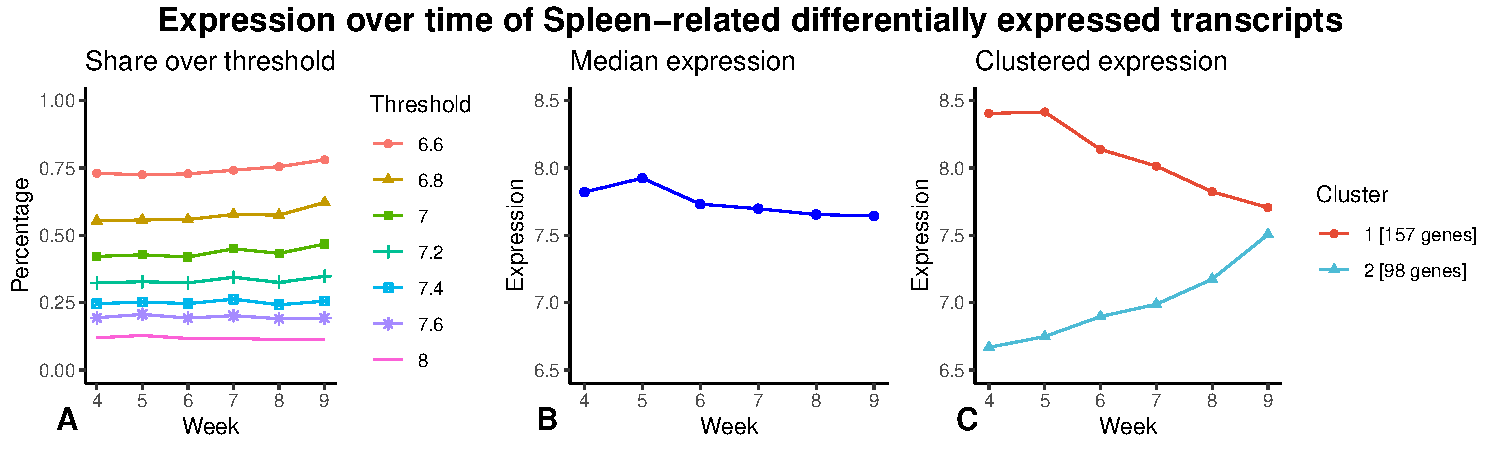
\includegraphics{Test2_files/figure-latex/unnamed-chunk-5-1.pdf}
\caption{A. For different expression thresholds the share of
differentially expressed transcripts with higher expressions than the
threshold is depicted. B. The median}
\end{figure}

\begin{figure}
\centering
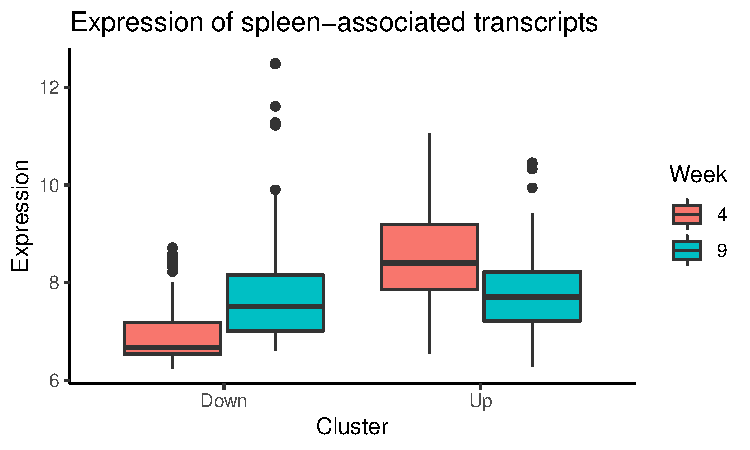
\includegraphics{Test2_files/figure-latex/unnamed-chunk-10-1.pdf}
\caption{A further look on the expression of transcripts in the up- and
downregulated clusters shows that the upregulated transcripts are close
to the minimum expression level between 6 and 7 in week 4 and showing
expressions between 7 and 8.5 by week 9. In contrast, the downregulated
genes have very high expression levels (8-9) by week 4 and decrease to a
more moderate expression between 7 and 8.5 analogous to the upregulated
transcripts.}
\end{figure}

\captionsetup[table]{labelformat=empty,skip=1pt}
\begin{longtable}{llllc}
\caption*{
{\large Spleen - Upregulated} \\ 
{\small List of differentially epxressed genes}
} \\ 
\toprule
Transcript & Gene & Protein & Summary & Expression\_over\_time \\ 
\midrule
ENST00000233505 & CENPA & centromere protein A & Member of the immunoglobulin superfamily & <?xml version='1.0' encoding='UTF-8' ?><svg xmlns='http://www.w3.org/2000/svg' xmlns:xlink='http://www.w3.org/1999/xlink' class='svglite' width='85.04pt' height='14.17pt' viewBox='0 0 85.04 14.17'><defs>  <style type='text/css'><![CDATA[    .svglite line, .svglite polyline, .svglite polygon, .svglite path, .svglite rect, .svglite circle {      fill: none;      stroke: #000000;      stroke-linecap: round;      stroke-linejoin: round;      stroke-miterlimit: 10.00;    }    .svglite text {      white-space: pre;    }  ]]></style></defs><rect width='100%' height='100%' style='stroke: none; fill: none;'/><defs>  <clipPath id='cpMC4wMHw4NS4wNHwwLjAwfDE0LjE3'>    <rect x='0.00' y='0.00' width='85.04' height='14.17' />  </clipPath></defs><g clip-path='url(#cpMC4wMHw4NS4wNHwwLjAwfDE0LjE3)'><line x1='11.86' y1='7.07' x2='65.18' y2='7.07' style='stroke-width: 0.21; stroke: #D3D3D3; stroke-linecap: butt;' /><line x1='11.86' y1='7.07' x2='65.18' y2='7.07' style='stroke-width: 0.21; stroke: #D3D3D3; stroke-linecap: butt;' /><line x1='11.86' y1='7.07' x2='65.18' y2='7.07' style='stroke-width: 0.21; stroke: #D3D3D3; stroke-linecap: butt;' /><line x1='11.86' y1='7.07' x2='65.18' y2='7.07' style='stroke-width: 0.21; stroke: #D3D3D3; stroke-linecap: butt;' /><line x1='11.86' y1='7.07' x2='65.18' y2='7.07' style='stroke-width: 0.21; stroke: #D3D3D3; stroke-linecap: butt;' /><line x1='11.86' y1='7.07' x2='65.18' y2='7.07' style='stroke-width: 0.21; stroke: #D3D3D3; stroke-linecap: butt;' /><text x='68.38' y='14.17' style='font-size: 5.69px; font-family: "Arial";' textLength='10.24px' lengthAdjust='spacingAndGlyphs'>7.6</text><polyline points='11.86,3.13 22.53,1.63 33.19,6.05 43.85,8.09 54.52,10.41 65.18,12.55 ' style='stroke-width: 1.07; stroke-linecap: butt;' /><circle cx='65.18' cy='12.55' r='0.89' style='stroke-width: 0.71; fill: #000000;' /><circle cx='65.18' cy='12.55' r='0.89' style='stroke-width: 0.71; stroke: #A020F0; fill: #A020F0;' /><circle cx='22.53' cy='1.63' r='0.89' style='stroke-width: 0.71; stroke: #00FF00; fill: #00FF00;' /></g></svg> \\ 
ENST00000247191 & DLGAP5 & DLG associated protein 5 & Mediates polarization of T cells and neutrophils & <?xml version='1.0' encoding='UTF-8' ?><svg xmlns='http://www.w3.org/2000/svg' xmlns:xlink='http://www.w3.org/1999/xlink' class='svglite' width='85.04pt' height='14.17pt' viewBox='0 0 85.04 14.17'><defs>  <style type='text/css'><![CDATA[    .svglite line, .svglite polyline, .svglite polygon, .svglite path, .svglite rect, .svglite circle {      fill: none;      stroke: #000000;      stroke-linecap: round;      stroke-linejoin: round;      stroke-miterlimit: 10.00;    }    .svglite text {      white-space: pre;    }  ]]></style></defs><rect width='100%' height='100%' style='stroke: none; fill: none;'/><defs>  <clipPath id='cpMC4wMHw4NS4wNHwwLjAwfDE0LjE3'>    <rect x='0.00' y='0.00' width='85.04' height='14.17' />  </clipPath></defs><g clip-path='url(#cpMC4wMHw4NS4wNHwwLjAwfDE0LjE3)'><line x1='11.86' y1='4.86' x2='65.18' y2='4.86' style='stroke-width: 0.21; stroke: #D3D3D3; stroke-linecap: butt;' /><line x1='11.86' y1='4.86' x2='65.18' y2='4.86' style='stroke-width: 0.21; stroke: #D3D3D3; stroke-linecap: butt;' /><line x1='11.86' y1='4.86' x2='65.18' y2='4.86' style='stroke-width: 0.21; stroke: #D3D3D3; stroke-linecap: butt;' /><line x1='11.86' y1='4.86' x2='65.18' y2='4.86' style='stroke-width: 0.21; stroke: #D3D3D3; stroke-linecap: butt;' /><line x1='11.86' y1='4.86' x2='65.18' y2='4.86' style='stroke-width: 0.21; stroke: #D3D3D3; stroke-linecap: butt;' /><line x1='11.86' y1='4.86' x2='65.18' y2='4.86' style='stroke-width: 0.21; stroke: #D3D3D3; stroke-linecap: butt;' /><text x='68.38' y='14.17' style='font-size: 5.69px; font-family: "Arial";' textLength='10.24px' lengthAdjust='spacingAndGlyphs'>8.3</text><polyline points='11.86,1.63 22.53,2.24 33.19,3.27 43.85,6.45 54.52,8.57 65.18,12.55 ' style='stroke-width: 1.07; stroke-linecap: butt;' /><circle cx='65.18' cy='12.55' r='0.89' style='stroke-width: 0.71; fill: #000000;' /><circle cx='65.18' cy='12.55' r='0.89' style='stroke-width: 0.71; stroke: #A020F0; fill: #A020F0;' /><circle cx='11.86' cy='1.63' r='0.89' style='stroke-width: 0.71; stroke: #00FF00; fill: #00FF00;' /></g></svg> \\ 
ENST00000247291 & AIF1L & allograft inflammatory factor 1 like & Secreted by cytptpxic lymphocytes & <?xml version='1.0' encoding='UTF-8' ?><svg xmlns='http://www.w3.org/2000/svg' xmlns:xlink='http://www.w3.org/1999/xlink' class='svglite' width='85.04pt' height='14.17pt' viewBox='0 0 85.04 14.17'><defs>  <style type='text/css'><![CDATA[    .svglite line, .svglite polyline, .svglite polygon, .svglite path, .svglite rect, .svglite circle {      fill: none;      stroke: #000000;      stroke-linecap: round;      stroke-linejoin: round;      stroke-miterlimit: 10.00;    }    .svglite text {      white-space: pre;    }  ]]></style></defs><rect width='100%' height='100%' style='stroke: none; fill: none;'/><defs>  <clipPath id='cpMC4wMHw4NS4wNHwwLjAwfDE0LjE3'>    <rect x='0.00' y='0.00' width='85.04' height='14.17' />  </clipPath></defs><g clip-path='url(#cpMC4wMHw4NS4wNHwwLjAwfDE0LjE3)'><line x1='11.86' y1='5.24' x2='65.18' y2='5.24' style='stroke-width: 0.21; stroke: #D3D3D3; stroke-linecap: butt;' /><line x1='11.86' y1='5.24' x2='65.18' y2='5.24' style='stroke-width: 0.21; stroke: #D3D3D3; stroke-linecap: butt;' /><line x1='11.86' y1='5.24' x2='65.18' y2='5.24' style='stroke-width: 0.21; stroke: #D3D3D3; stroke-linecap: butt;' /><line x1='11.86' y1='5.24' x2='65.18' y2='5.24' style='stroke-width: 0.21; stroke: #D3D3D3; stroke-linecap: butt;' /><line x1='11.86' y1='5.24' x2='65.18' y2='5.24' style='stroke-width: 0.21; stroke: #D3D3D3; stroke-linecap: butt;' /><line x1='11.86' y1='5.24' x2='65.18' y2='5.24' style='stroke-width: 0.21; stroke: #D3D3D3; stroke-linecap: butt;' /><text x='68.38' y='14.17' style='font-size: 5.69px; font-family: "Arial";' textLength='10.24px' lengthAdjust='spacingAndGlyphs'>7.2</text><polyline points='11.86,5.46 22.53,1.63 33.19,5.02 43.85,4.04 54.52,9.44 65.18,12.55 ' style='stroke-width: 1.07; stroke-linecap: butt;' /><circle cx='65.18' cy='12.55' r='0.89' style='stroke-width: 0.71; fill: #000000;' /><circle cx='65.18' cy='12.55' r='0.89' style='stroke-width: 0.71; stroke: #A020F0; fill: #A020F0;' /><circle cx='22.53' cy='1.63' r='0.89' style='stroke-width: 0.71; stroke: #00FF00; fill: #00FF00;' /></g></svg> \\ 
ENST00000260359 & NUSAP1 & nucleolar and spindle associated protein 1 & Can upregulate blood pressure & <?xml version='1.0' encoding='UTF-8' ?><svg xmlns='http://www.w3.org/2000/svg' xmlns:xlink='http://www.w3.org/1999/xlink' class='svglite' width='85.04pt' height='14.17pt' viewBox='0 0 85.04 14.17'><defs>  <style type='text/css'><![CDATA[    .svglite line, .svglite polyline, .svglite polygon, .svglite path, .svglite rect, .svglite circle {      fill: none;      stroke: #000000;      stroke-linecap: round;      stroke-linejoin: round;      stroke-miterlimit: 10.00;    }    .svglite text {      white-space: pre;    }  ]]></style></defs><rect width='100%' height='100%' style='stroke: none; fill: none;'/><defs>  <clipPath id='cpMC4wMHw4NS4wNHwwLjAwfDE0LjE3'>    <rect x='0.00' y='0.00' width='85.04' height='14.17' />  </clipPath></defs><g clip-path='url(#cpMC4wMHw4NS4wNHwwLjAwfDE0LjE3)'><line x1='11.86' y1='5.95' x2='65.18' y2='5.95' style='stroke-width: 0.21; stroke: #D3D3D3; stroke-linecap: butt;' /><line x1='11.86' y1='5.95' x2='65.18' y2='5.95' style='stroke-width: 0.21; stroke: #D3D3D3; stroke-linecap: butt;' /><line x1='11.86' y1='5.95' x2='65.18' y2='5.95' style='stroke-width: 0.21; stroke: #D3D3D3; stroke-linecap: butt;' /><line x1='11.86' y1='5.95' x2='65.18' y2='5.95' style='stroke-width: 0.21; stroke: #D3D3D3; stroke-linecap: butt;' /><line x1='11.86' y1='5.95' x2='65.18' y2='5.95' style='stroke-width: 0.21; stroke: #D3D3D3; stroke-linecap: butt;' /><line x1='11.86' y1='5.95' x2='65.18' y2='5.95' style='stroke-width: 0.21; stroke: #D3D3D3; stroke-linecap: butt;' /><text x='68.38' y='14.17' style='font-size: 5.69px; font-family: "Arial";' textLength='10.24px' lengthAdjust='spacingAndGlyphs'>8.6</text><polyline points='11.86,1.63 22.53,1.97 33.19,5.49 43.85,6.42 54.52,8.34 65.18,12.55 ' style='stroke-width: 1.07; stroke-linecap: butt;' /><circle cx='65.18' cy='12.55' r='0.89' style='stroke-width: 0.71; fill: #000000;' /><circle cx='65.18' cy='12.55' r='0.89' style='stroke-width: 0.71; stroke: #A020F0; fill: #A020F0;' /><circle cx='11.86' cy='1.63' r='0.89' style='stroke-width: 0.71; stroke: #00FF00; fill: #00FF00;' /></g></svg> \\ 
ENST00000263201 & CDC45 & cell division cycle 45 & B lymphocyte chemoattractant & <?xml version='1.0' encoding='UTF-8' ?><svg xmlns='http://www.w3.org/2000/svg' xmlns:xlink='http://www.w3.org/1999/xlink' class='svglite' width='85.04pt' height='14.17pt' viewBox='0 0 85.04 14.17'><defs>  <style type='text/css'><![CDATA[    .svglite line, .svglite polyline, .svglite polygon, .svglite path, .svglite rect, .svglite circle {      fill: none;      stroke: #000000;      stroke-linecap: round;      stroke-linejoin: round;      stroke-miterlimit: 10.00;    }    .svglite text {      white-space: pre;    }  ]]></style></defs><rect width='100%' height='100%' style='stroke: none; fill: none;'/><defs>  <clipPath id='cpMC4wMHw4NS4wNHwwLjAwfDE0LjE3'>    <rect x='0.00' y='0.00' width='85.04' height='14.17' />  </clipPath></defs><g clip-path='url(#cpMC4wMHw4NS4wNHwwLjAwfDE0LjE3)'><line x1='11.86' y1='8.82' x2='65.18' y2='8.82' style='stroke-width: 0.21; stroke: #D3D3D3; stroke-linecap: butt;' /><line x1='11.86' y1='8.82' x2='65.18' y2='8.82' style='stroke-width: 0.21; stroke: #D3D3D3; stroke-linecap: butt;' /><line x1='11.86' y1='8.82' x2='65.18' y2='8.82' style='stroke-width: 0.21; stroke: #D3D3D3; stroke-linecap: butt;' /><line x1='11.86' y1='8.82' x2='65.18' y2='8.82' style='stroke-width: 0.21; stroke: #D3D3D3; stroke-linecap: butt;' /><line x1='11.86' y1='8.82' x2='65.18' y2='8.82' style='stroke-width: 0.21; stroke: #D3D3D3; stroke-linecap: butt;' /><line x1='11.86' y1='8.82' x2='65.18' y2='8.82' style='stroke-width: 0.21; stroke: #D3D3D3; stroke-linecap: butt;' /><text x='68.38' y='14.17' style='font-size: 5.69px; font-family: "Arial";' textLength='10.24px' lengthAdjust='spacingAndGlyphs'>7.3</text><polyline points='11.86,8.39 22.53,1.63 33.19,8.40 43.85,9.25 54.52,11.17 65.18,12.55 ' style='stroke-width: 1.07; stroke-linecap: butt;' /><circle cx='65.18' cy='12.55' r='0.89' style='stroke-width: 0.71; fill: #000000;' /><circle cx='65.18' cy='12.55' r='0.89' style='stroke-width: 0.71; stroke: #A020F0; fill: #A020F0;' /><circle cx='22.53' cy='1.63' r='0.89' style='stroke-width: 0.71; stroke: #00FF00; fill: #00FF00;' /></g></svg> \\ 
ENST00000296289 & NA & NA & IL-11 receptor & <?xml version='1.0' encoding='UTF-8' ?><svg xmlns='http://www.w3.org/2000/svg' xmlns:xlink='http://www.w3.org/1999/xlink' class='svglite' width='85.04pt' height='14.17pt' viewBox='0 0 85.04 14.17'><defs>  <style type='text/css'><![CDATA[    .svglite line, .svglite polyline, .svglite polygon, .svglite path, .svglite rect, .svglite circle {      fill: none;      stroke: #000000;      stroke-linecap: round;      stroke-linejoin: round;      stroke-miterlimit: 10.00;    }    .svglite text {      white-space: pre;    }  ]]></style></defs><rect width='100%' height='100%' style='stroke: none; fill: none;'/><defs>  <clipPath id='cpMC4wMHw4NS4wNHwwLjAwfDE0LjE3'>    <rect x='0.00' y='0.00' width='85.04' height='14.17' />  </clipPath></defs><g clip-path='url(#cpMC4wMHw4NS4wNHwwLjAwfDE0LjE3)'><line x1='11.86' y1='5.95' x2='65.18' y2='5.95' style='stroke-width: 0.21; stroke: #D3D3D3; stroke-linecap: butt;' /><line x1='11.86' y1='5.95' x2='65.18' y2='5.95' style='stroke-width: 0.21; stroke: #D3D3D3; stroke-linecap: butt;' /><line x1='11.86' y1='5.95' x2='65.18' y2='5.95' style='stroke-width: 0.21; stroke: #D3D3D3; stroke-linecap: butt;' /><line x1='11.86' y1='5.95' x2='65.18' y2='5.95' style='stroke-width: 0.21; stroke: #D3D3D3; stroke-linecap: butt;' /><line x1='11.86' y1='5.95' x2='65.18' y2='5.95' style='stroke-width: 0.21; stroke: #D3D3D3; stroke-linecap: butt;' /><line x1='11.86' y1='5.95' x2='65.18' y2='5.95' style='stroke-width: 0.21; stroke: #D3D3D3; stroke-linecap: butt;' /><text x='68.38' y='14.17' style='font-size: 5.69px; font-family: "Arial";' textLength='10.24px' lengthAdjust='spacingAndGlyphs'>8.6</text><polyline points='11.86,1.63 22.53,3.41 33.19,6.81 43.85,5.09 54.52,12.50 65.18,12.55 ' style='stroke-width: 1.07; stroke-linecap: butt;' /><circle cx='65.18' cy='12.55' r='0.89' style='stroke-width: 0.71; fill: #000000;' /><circle cx='65.18' cy='12.55' r='0.89' style='stroke-width: 0.71; stroke: #A020F0; fill: #A020F0;' /><circle cx='11.86' cy='1.63' r='0.89' style='stroke-width: 0.71; stroke: #00FF00; fill: #00FF00;' /></g></svg> \\ 
ENST00000300093 & PLK1 & polo like kinase 1 &  & <?xml version='1.0' encoding='UTF-8' ?><svg xmlns='http://www.w3.org/2000/svg' xmlns:xlink='http://www.w3.org/1999/xlink' class='svglite' width='85.04pt' height='14.17pt' viewBox='0 0 85.04 14.17'><defs>  <style type='text/css'><![CDATA[    .svglite line, .svglite polyline, .svglite polygon, .svglite path, .svglite rect, .svglite circle {      fill: none;      stroke: #000000;      stroke-linecap: round;      stroke-linejoin: round;      stroke-miterlimit: 10.00;    }    .svglite text {      white-space: pre;    }  ]]></style></defs><rect width='100%' height='100%' style='stroke: none; fill: none;'/><defs>  <clipPath id='cpMC4wMHw4NS4wNHwwLjAwfDE0LjE3'>    <rect x='0.00' y='0.00' width='85.04' height='14.17' />  </clipPath></defs><g clip-path='url(#cpMC4wMHw4NS4wNHwwLjAwfDE0LjE3)'><line x1='11.86' y1='7.46' x2='65.18' y2='7.46' style='stroke-width: 0.21; stroke: #D3D3D3; stroke-linecap: butt;' /><line x1='11.86' y1='7.46' x2='65.18' y2='7.46' style='stroke-width: 0.21; stroke: #D3D3D3; stroke-linecap: butt;' /><line x1='11.86' y1='7.46' x2='65.18' y2='7.46' style='stroke-width: 0.21; stroke: #D3D3D3; stroke-linecap: butt;' /><line x1='11.86' y1='7.46' x2='65.18' y2='7.46' style='stroke-width: 0.21; stroke: #D3D3D3; stroke-linecap: butt;' /><line x1='11.86' y1='7.46' x2='65.18' y2='7.46' style='stroke-width: 0.21; stroke: #D3D3D3; stroke-linecap: butt;' /><line x1='11.86' y1='7.46' x2='65.18' y2='7.46' style='stroke-width: 0.21; stroke: #D3D3D3; stroke-linecap: butt;' /><text x='68.38' y='13.34' style='font-size: 5.69px; font-family: "Arial";' textLength='10.24px' lengthAdjust='spacingAndGlyphs'>7.7</text><polyline points='11.86,1.63 22.53,2.11 33.19,6.79 43.85,8.14 54.52,12.55 65.18,11.72 ' style='stroke-width: 1.07; stroke-linecap: butt;' /><circle cx='65.18' cy='11.72' r='0.89' style='stroke-width: 0.71; fill: #000000;' /><circle cx='54.52' cy='12.55' r='0.89' style='stroke-width: 0.71; stroke: #A020F0; fill: #A020F0;' /><circle cx='11.86' cy='1.63' r='0.89' style='stroke-width: 0.71; stroke: #00FF00; fill: #00FF00;' /></g></svg> \\ 
ENST00000313093 & ARHGAP45 & Rho GTPase activating protein 45 & Contains von Willebrand factor domains & <?xml version='1.0' encoding='UTF-8' ?><svg xmlns='http://www.w3.org/2000/svg' xmlns:xlink='http://www.w3.org/1999/xlink' class='svglite' width='85.04pt' height='14.17pt' viewBox='0 0 85.04 14.17'><defs>  <style type='text/css'><![CDATA[    .svglite line, .svglite polyline, .svglite polygon, .svglite path, .svglite rect, .svglite circle {      fill: none;      stroke: #000000;      stroke-linecap: round;      stroke-linejoin: round;      stroke-miterlimit: 10.00;    }    .svglite text {      white-space: pre;    }  ]]></style></defs><rect width='100%' height='100%' style='stroke: none; fill: none;'/><defs>  <clipPath id='cpMC4wMHw4NS4wNHwwLjAwfDE0LjE3'>    <rect x='0.00' y='0.00' width='85.04' height='14.17' />  </clipPath></defs><g clip-path='url(#cpMC4wMHw4NS4wNHwwLjAwfDE0LjE3)'><line x1='11.86' y1='12.29' x2='65.18' y2='12.29' style='stroke-width: 0.21; stroke: #D3D3D3; stroke-linecap: butt;' /><line x1='11.86' y1='12.29' x2='65.18' y2='12.29' style='stroke-width: 0.21; stroke: #D3D3D3; stroke-linecap: butt;' /><line x1='11.86' y1='12.29' x2='65.18' y2='12.29' style='stroke-width: 0.21; stroke: #D3D3D3; stroke-linecap: butt;' /><line x1='11.86' y1='12.29' x2='65.18' y2='12.29' style='stroke-width: 0.21; stroke: #D3D3D3; stroke-linecap: butt;' /><line x1='11.86' y1='12.29' x2='65.18' y2='12.29' style='stroke-width: 0.21; stroke: #D3D3D3; stroke-linecap: butt;' /><line x1='11.86' y1='12.29' x2='65.18' y2='12.29' style='stroke-width: 0.21; stroke: #D3D3D3; stroke-linecap: butt;' /><text x='68.38' y='14.01' style='font-size: 5.69px; font-family: "Arial";' textLength='10.24px' lengthAdjust='spacingAndGlyphs'>6.9</text><polyline points='11.86,1.63 22.53,9.23 33.19,12.55 43.85,12.21 54.52,12.37 65.18,12.39 ' style='stroke-width: 1.07; stroke-linecap: butt;' /><circle cx='65.18' cy='12.39' r='0.89' style='stroke-width: 0.71; fill: #000000;' /><circle cx='33.19' cy='12.55' r='0.89' style='stroke-width: 0.71; stroke: #A020F0; fill: #A020F0;' /><circle cx='11.86' cy='1.63' r='0.89' style='stroke-width: 0.71; stroke: #00FF00; fill: #00FF00;' /></g></svg> \\ 
ENST00000327331 & CDCA8 & cell division cycle associated 8 & May function as a cytokine & <?xml version='1.0' encoding='UTF-8' ?><svg xmlns='http://www.w3.org/2000/svg' xmlns:xlink='http://www.w3.org/1999/xlink' class='svglite' width='85.04pt' height='14.17pt' viewBox='0 0 85.04 14.17'><defs>  <style type='text/css'><![CDATA[    .svglite line, .svglite polyline, .svglite polygon, .svglite path, .svglite rect, .svglite circle {      fill: none;      stroke: #000000;      stroke-linecap: round;      stroke-linejoin: round;      stroke-miterlimit: 10.00;    }    .svglite text {      white-space: pre;    }  ]]></style></defs><rect width='100%' height='100%' style='stroke: none; fill: none;'/><defs>  <clipPath id='cpMC4wMHw4NS4wNHwwLjAwfDE0LjE3'>    <rect x='0.00' y='0.00' width='85.04' height='14.17' />  </clipPath></defs><g clip-path='url(#cpMC4wMHw4NS4wNHwwLjAwfDE0LjE3)'><line x1='11.86' y1='7.12' x2='65.18' y2='7.12' style='stroke-width: 0.21; stroke: #D3D3D3; stroke-linecap: butt;' /><line x1='11.86' y1='7.12' x2='65.18' y2='7.12' style='stroke-width: 0.21; stroke: #D3D3D3; stroke-linecap: butt;' /><line x1='11.86' y1='7.12' x2='65.18' y2='7.12' style='stroke-width: 0.21; stroke: #D3D3D3; stroke-linecap: butt;' /><line x1='11.86' y1='7.12' x2='65.18' y2='7.12' style='stroke-width: 0.21; stroke: #D3D3D3; stroke-linecap: butt;' /><line x1='11.86' y1='7.12' x2='65.18' y2='7.12' style='stroke-width: 0.21; stroke: #D3D3D3; stroke-linecap: butt;' /><line x1='11.86' y1='7.12' x2='65.18' y2='7.12' style='stroke-width: 0.21; stroke: #D3D3D3; stroke-linecap: butt;' /><text x='68.38' y='14.17' style='font-size: 5.69px; font-family: "Arial";' textLength='10.24px' lengthAdjust='spacingAndGlyphs'>7.8</text><polyline points='11.86,3.46 22.53,1.63 33.19,6.31 43.85,7.92 54.52,11.75 65.18,12.55 ' style='stroke-width: 1.07; stroke-linecap: butt;' /><circle cx='65.18' cy='12.55' r='0.89' style='stroke-width: 0.71; fill: #000000;' /><circle cx='65.18' cy='12.55' r='0.89' style='stroke-width: 0.71; stroke: #A020F0; fill: #A020F0;' /><circle cx='22.53' cy='1.63' r='0.89' style='stroke-width: 0.71; stroke: #00FF00; fill: #00FF00;' /></g></svg> \\ 
ENST00000338631 & ACIN1 & apoptotic chromatin condensation inducer 1 & Plays a role in immune surveillance & <?xml version='1.0' encoding='UTF-8' ?><svg xmlns='http://www.w3.org/2000/svg' xmlns:xlink='http://www.w3.org/1999/xlink' class='svglite' width='85.04pt' height='14.17pt' viewBox='0 0 85.04 14.17'><defs>  <style type='text/css'><![CDATA[    .svglite line, .svglite polyline, .svglite polygon, .svglite path, .svglite rect, .svglite circle {      fill: none;      stroke: #000000;      stroke-linecap: round;      stroke-linejoin: round;      stroke-miterlimit: 10.00;    }    .svglite text {      white-space: pre;    }  ]]></style></defs><rect width='100%' height='100%' style='stroke: none; fill: none;'/><defs>  <clipPath id='cpMC4wMHw4NS4wNHwwLjAwfDE0LjE3'>    <rect x='0.00' y='0.00' width='85.04' height='14.17' />  </clipPath></defs><g clip-path='url(#cpMC4wMHw4NS4wNHwwLjAwfDE0LjE3)'><line x1='11.86' y1='5.45' x2='65.18' y2='5.45' style='stroke-width: 0.21; stroke: #D3D3D3; stroke-linecap: butt;' /><line x1='11.86' y1='5.45' x2='65.18' y2='5.45' style='stroke-width: 0.21; stroke: #D3D3D3; stroke-linecap: butt;' /><line x1='11.86' y1='5.45' x2='65.18' y2='5.45' style='stroke-width: 0.21; stroke: #D3D3D3; stroke-linecap: butt;' /><line x1='11.86' y1='5.45' x2='65.18' y2='5.45' style='stroke-width: 0.21; stroke: #D3D3D3; stroke-linecap: butt;' /><line x1='11.86' y1='5.45' x2='65.18' y2='5.45' style='stroke-width: 0.21; stroke: #D3D3D3; stroke-linecap: butt;' /><line x1='11.86' y1='5.45' x2='65.18' y2='5.45' style='stroke-width: 0.21; stroke: #D3D3D3; stroke-linecap: butt;' /><text x='68.38' y='14.17' style='font-size: 5.69px; font-family: "Arial";' textLength='10.24px' lengthAdjust='spacingAndGlyphs'>7.9</text><polyline points='11.86,5.29 22.53,1.63 33.19,5.62 43.85,3.22 54.52,11.93 65.18,12.55 ' style='stroke-width: 1.07; stroke-linecap: butt;' /><circle cx='65.18' cy='12.55' r='0.89' style='stroke-width: 0.71; fill: #000000;' /><circle cx='65.18' cy='12.55' r='0.89' style='stroke-width: 0.71; stroke: #A020F0; fill: #A020F0;' /><circle cx='22.53' cy='1.63' r='0.89' style='stroke-width: 0.71; stroke: #00FF00; fill: #00FF00;' /></g></svg> \\ 
ENST00000349718 & CMTM7 & CKLF like MARVEL transmembrane domain containing 7 & Regulating the complement cascade & <?xml version='1.0' encoding='UTF-8' ?><svg xmlns='http://www.w3.org/2000/svg' xmlns:xlink='http://www.w3.org/1999/xlink' class='svglite' width='85.04pt' height='14.17pt' viewBox='0 0 85.04 14.17'><defs>  <style type='text/css'><![CDATA[    .svglite line, .svglite polyline, .svglite polygon, .svglite path, .svglite rect, .svglite circle {      fill: none;      stroke: #000000;      stroke-linecap: round;      stroke-linejoin: round;      stroke-miterlimit: 10.00;    }    .svglite text {      white-space: pre;    }  ]]></style></defs><rect width='100%' height='100%' style='stroke: none; fill: none;'/><defs>  <clipPath id='cpMC4wMHw4NS4wNHwwLjAwfDE0LjE3'>    <rect x='0.00' y='0.00' width='85.04' height='14.17' />  </clipPath></defs><g clip-path='url(#cpMC4wMHw4NS4wNHwwLjAwfDE0LjE3)'><line x1='11.86' y1='9.38' x2='65.18' y2='9.38' style='stroke-width: 0.21; stroke: #D3D3D3; stroke-linecap: butt;' /><line x1='11.86' y1='9.38' x2='65.18' y2='9.38' style='stroke-width: 0.21; stroke: #D3D3D3; stroke-linecap: butt;' /><line x1='11.86' y1='9.38' x2='65.18' y2='9.38' style='stroke-width: 0.21; stroke: #D3D3D3; stroke-linecap: butt;' /><line x1='11.86' y1='9.38' x2='65.18' y2='9.38' style='stroke-width: 0.21; stroke: #D3D3D3; stroke-linecap: butt;' /><line x1='11.86' y1='9.38' x2='65.18' y2='9.38' style='stroke-width: 0.21; stroke: #D3D3D3; stroke-linecap: butt;' /><line x1='11.86' y1='9.38' x2='65.18' y2='9.38' style='stroke-width: 0.21; stroke: #D3D3D3; stroke-linecap: butt;' /><text x='68.38' y='14.17' style='font-size: 5.69px; font-family: "Arial";' textLength='10.24px' lengthAdjust='spacingAndGlyphs'>7.6</text><polyline points='11.86,1.63 22.53,4.62 33.19,9.29 43.85,9.46 54.52,10.65 65.18,12.55 ' style='stroke-width: 1.07; stroke-linecap: butt;' /><circle cx='65.18' cy='12.55' r='0.89' style='stroke-width: 0.71; fill: #000000;' /><circle cx='65.18' cy='12.55' r='0.89' style='stroke-width: 0.71; stroke: #A020F0; fill: #A020F0;' /><circle cx='11.86' cy='1.63' r='0.89' style='stroke-width: 0.71; stroke: #00FF00; fill: #00FF00;' /></g></svg> \\ 
ENST00000352331 & KIF23 & kinesin family member 23 & HLA class II & <?xml version='1.0' encoding='UTF-8' ?><svg xmlns='http://www.w3.org/2000/svg' xmlns:xlink='http://www.w3.org/1999/xlink' class='svglite' width='85.04pt' height='14.17pt' viewBox='0 0 85.04 14.17'><defs>  <style type='text/css'><![CDATA[    .svglite line, .svglite polyline, .svglite polygon, .svglite path, .svglite rect, .svglite circle {      fill: none;      stroke: #000000;      stroke-linecap: round;      stroke-linejoin: round;      stroke-miterlimit: 10.00;    }    .svglite text {      white-space: pre;    }  ]]></style></defs><rect width='100%' height='100%' style='stroke: none; fill: none;'/><defs>  <clipPath id='cpMC4wMHw4NS4wNHwwLjAwfDE0LjE3'>    <rect x='0.00' y='0.00' width='85.04' height='14.17' />  </clipPath></defs><g clip-path='url(#cpMC4wMHw4NS4wNHwwLjAwfDE0LjE3)'><line x1='11.86' y1='7.28' x2='65.18' y2='7.28' style='stroke-width: 0.21; stroke: #D3D3D3; stroke-linecap: butt;' /><line x1='11.86' y1='7.28' x2='65.18' y2='7.28' style='stroke-width: 0.21; stroke: #D3D3D3; stroke-linecap: butt;' /><line x1='11.86' y1='7.28' x2='65.18' y2='7.28' style='stroke-width: 0.21; stroke: #D3D3D3; stroke-linecap: butt;' /><line x1='11.86' y1='7.28' x2='65.18' y2='7.28' style='stroke-width: 0.21; stroke: #D3D3D3; stroke-linecap: butt;' /><line x1='11.86' y1='7.28' x2='65.18' y2='7.28' style='stroke-width: 0.21; stroke: #D3D3D3; stroke-linecap: butt;' /><line x1='11.86' y1='7.28' x2='65.18' y2='7.28' style='stroke-width: 0.21; stroke: #D3D3D3; stroke-linecap: butt;' /><text x='68.38' y='14.17' style='font-size: 5.69px; font-family: "Arial";' textLength='10.24px' lengthAdjust='spacingAndGlyphs'>7.7</text><polyline points='11.86,3.62 22.53,1.63 33.19,5.34 43.85,9.22 54.52,10.87 65.18,12.55 ' style='stroke-width: 1.07; stroke-linecap: butt;' /><circle cx='65.18' cy='12.55' r='0.89' style='stroke-width: 0.71; fill: #000000;' /><circle cx='65.18' cy='12.55' r='0.89' style='stroke-width: 0.71; stroke: #A020F0; fill: #A020F0;' /><circle cx='22.53' cy='1.63' r='0.89' style='stroke-width: 0.71; stroke: #00FF00; fill: #00FF00;' /></g></svg> \\ 
ENST00000357481 & ACIN1 & apoptotic chromatin condensation inducer 1 & Endocytosis of pathogen & <?xml version='1.0' encoding='UTF-8' ?><svg xmlns='http://www.w3.org/2000/svg' xmlns:xlink='http://www.w3.org/1999/xlink' class='svglite' width='85.04pt' height='14.17pt' viewBox='0 0 85.04 14.17'><defs>  <style type='text/css'><![CDATA[    .svglite line, .svglite polyline, .svglite polygon, .svglite path, .svglite rect, .svglite circle {      fill: none;      stroke: #000000;      stroke-linecap: round;      stroke-linejoin: round;      stroke-miterlimit: 10.00;    }    .svglite text {      white-space: pre;    }  ]]></style></defs><rect width='100%' height='100%' style='stroke: none; fill: none;'/><defs>  <clipPath id='cpMC4wMHw4NS4wNHwwLjAwfDE0LjE3'>    <rect x='0.00' y='0.00' width='85.04' height='14.17' />  </clipPath></defs><g clip-path='url(#cpMC4wMHw4NS4wNHwwLjAwfDE0LjE3)'><line x1='11.86' y1='5.45' x2='65.18' y2='5.45' style='stroke-width: 0.21; stroke: #D3D3D3; stroke-linecap: butt;' /><line x1='11.86' y1='5.45' x2='65.18' y2='5.45' style='stroke-width: 0.21; stroke: #D3D3D3; stroke-linecap: butt;' /><line x1='11.86' y1='5.45' x2='65.18' y2='5.45' style='stroke-width: 0.21; stroke: #D3D3D3; stroke-linecap: butt;' /><line x1='11.86' y1='5.45' x2='65.18' y2='5.45' style='stroke-width: 0.21; stroke: #D3D3D3; stroke-linecap: butt;' /><line x1='11.86' y1='5.45' x2='65.18' y2='5.45' style='stroke-width: 0.21; stroke: #D3D3D3; stroke-linecap: butt;' /><line x1='11.86' y1='5.45' x2='65.18' y2='5.45' style='stroke-width: 0.21; stroke: #D3D3D3; stroke-linecap: butt;' /><text x='68.38' y='14.17' style='font-size: 5.69px; font-family: "Arial";' textLength='10.24px' lengthAdjust='spacingAndGlyphs'>7.9</text><polyline points='11.86,5.29 22.53,1.63 33.19,5.62 43.85,3.22 54.52,11.93 65.18,12.55 ' style='stroke-width: 1.07; stroke-linecap: butt;' /><circle cx='65.18' cy='12.55' r='0.89' style='stroke-width: 0.71; fill: #000000;' /><circle cx='65.18' cy='12.55' r='0.89' style='stroke-width: 0.71; stroke: #A020F0; fill: #A020F0;' /><circle cx='22.53' cy='1.63' r='0.89' style='stroke-width: 0.71; stroke: #00FF00; fill: #00FF00;' /></g></svg> \\ 
ENST00000357886 & CDK5RAP1 & CDK5 regulatory subunit associated protein 1 & Receptors for interferons alpha and beta & <?xml version='1.0' encoding='UTF-8' ?><svg xmlns='http://www.w3.org/2000/svg' xmlns:xlink='http://www.w3.org/1999/xlink' class='svglite' width='85.04pt' height='14.17pt' viewBox='0 0 85.04 14.17'><defs>  <style type='text/css'><![CDATA[    .svglite line, .svglite polyline, .svglite polygon, .svglite path, .svglite rect, .svglite circle {      fill: none;      stroke: #000000;      stroke-linecap: round;      stroke-linejoin: round;      stroke-miterlimit: 10.00;    }    .svglite text {      white-space: pre;    }  ]]></style></defs><rect width='100%' height='100%' style='stroke: none; fill: none;'/><defs>  <clipPath id='cpMC4wMHw4NS4wNHwwLjAwfDE0LjE3'>    <rect x='0.00' y='0.00' width='85.04' height='14.17' />  </clipPath></defs><g clip-path='url(#cpMC4wMHw4NS4wNHwwLjAwfDE0LjE3)'><line x1='11.86' y1='6.38' x2='65.18' y2='6.38' style='stroke-width: 0.21; stroke: #D3D3D3; stroke-linecap: butt;' /><line x1='11.86' y1='6.38' x2='65.18' y2='6.38' style='stroke-width: 0.21; stroke: #D3D3D3; stroke-linecap: butt;' /><line x1='11.86' y1='6.38' x2='65.18' y2='6.38' style='stroke-width: 0.21; stroke: #D3D3D3; stroke-linecap: butt;' /><line x1='11.86' y1='6.38' x2='65.18' y2='6.38' style='stroke-width: 0.21; stroke: #D3D3D3; stroke-linecap: butt;' /><line x1='11.86' y1='6.38' x2='65.18' y2='6.38' style='stroke-width: 0.21; stroke: #D3D3D3; stroke-linecap: butt;' /><line x1='11.86' y1='6.38' x2='65.18' y2='6.38' style='stroke-width: 0.21; stroke: #D3D3D3; stroke-linecap: butt;' /><text x='68.38' y='14.17' style='font-size: 5.69px; font-family: "Arial";' textLength='10.24px' lengthAdjust='spacingAndGlyphs'>7.6</text><polyline points='11.86,1.63 22.53,2.49 33.19,4.77 43.85,7.98 54.52,10.42 65.18,12.55 ' style='stroke-width: 1.07; stroke-linecap: butt;' /><circle cx='65.18' cy='12.55' r='0.89' style='stroke-width: 0.71; fill: #000000;' /><circle cx='65.18' cy='12.55' r='0.89' style='stroke-width: 0.71; stroke: #A020F0; fill: #A020F0;' /><circle cx='11.86' cy='1.63' r='0.89' style='stroke-width: 0.71; stroke: #00FF00; fill: #00FF00;' /></g></svg> \\ 
ENST00000371485 & CEP55 & centrosomal protein 55 & Fibroblast growth factor & <?xml version='1.0' encoding='UTF-8' ?><svg xmlns='http://www.w3.org/2000/svg' xmlns:xlink='http://www.w3.org/1999/xlink' class='svglite' width='85.04pt' height='14.17pt' viewBox='0 0 85.04 14.17'><defs>  <style type='text/css'><![CDATA[    .svglite line, .svglite polyline, .svglite polygon, .svglite path, .svglite rect, .svglite circle {      fill: none;      stroke: #000000;      stroke-linecap: round;      stroke-linejoin: round;      stroke-miterlimit: 10.00;    }    .svglite text {      white-space: pre;    }  ]]></style></defs><rect width='100%' height='100%' style='stroke: none; fill: none;'/><defs>  <clipPath id='cpMC4wMHw4NS4wNHwwLjAwfDE0LjE3'>    <rect x='0.00' y='0.00' width='85.04' height='14.17' />  </clipPath></defs><g clip-path='url(#cpMC4wMHw4NS4wNHwwLjAwfDE0LjE3)'><line x1='11.86' y1='7.40' x2='65.18' y2='7.40' style='stroke-width: 0.21; stroke: #D3D3D3; stroke-linecap: butt;' /><line x1='11.86' y1='7.40' x2='65.18' y2='7.40' style='stroke-width: 0.21; stroke: #D3D3D3; stroke-linecap: butt;' /><line x1='11.86' y1='7.40' x2='65.18' y2='7.40' style='stroke-width: 0.21; stroke: #D3D3D3; stroke-linecap: butt;' /><line x1='11.86' y1='7.40' x2='65.18' y2='7.40' style='stroke-width: 0.21; stroke: #D3D3D3; stroke-linecap: butt;' /><line x1='11.86' y1='7.40' x2='65.18' y2='7.40' style='stroke-width: 0.21; stroke: #D3D3D3; stroke-linecap: butt;' /><line x1='11.86' y1='7.40' x2='65.18' y2='7.40' style='stroke-width: 0.21; stroke: #D3D3D3; stroke-linecap: butt;' /><text x='68.38' y='13.97' style='font-size: 5.69px; font-family: "Arial";' textLength='10.24px' lengthAdjust='spacingAndGlyphs'>7.1</text><polyline points='11.86,4.72 22.53,1.63 33.19,3.21 43.85,12.55 54.52,10.08 65.18,12.34 ' style='stroke-width: 1.07; stroke-linecap: butt;' /><circle cx='65.18' cy='12.34' r='0.89' style='stroke-width: 0.71; fill: #000000;' /><circle cx='43.85' cy='12.55' r='0.89' style='stroke-width: 0.71; stroke: #A020F0; fill: #A020F0;' /><circle cx='22.53' cy='1.63' r='0.89' style='stroke-width: 0.71; stroke: #00FF00; fill: #00FF00;' /></g></svg> \\ 
ENST00000411486 & HJURP & Holliday junction recognition protein & Regulating the complement cascade & <?xml version='1.0' encoding='UTF-8' ?><svg xmlns='http://www.w3.org/2000/svg' xmlns:xlink='http://www.w3.org/1999/xlink' class='svglite' width='85.04pt' height='14.17pt' viewBox='0 0 85.04 14.17'><defs>  <style type='text/css'><![CDATA[    .svglite line, .svglite polyline, .svglite polygon, .svglite path, .svglite rect, .svglite circle {      fill: none;      stroke: #000000;      stroke-linecap: round;      stroke-linejoin: round;      stroke-miterlimit: 10.00;    }    .svglite text {      white-space: pre;    }  ]]></style></defs><rect width='100%' height='100%' style='stroke: none; fill: none;'/><defs>  <clipPath id='cpMC4wMHw4NS4wNHwwLjAwfDE0LjE3'>    <rect x='0.00' y='0.00' width='85.04' height='14.17' />  </clipPath></defs><g clip-path='url(#cpMC4wMHw4NS4wNHwwLjAwfDE0LjE3)'><line x1='11.86' y1='6.11' x2='65.18' y2='6.11' style='stroke-width: 0.21; stroke: #D3D3D3; stroke-linecap: butt;' /><line x1='11.86' y1='6.11' x2='65.18' y2='6.11' style='stroke-width: 0.21; stroke: #D3D3D3; stroke-linecap: butt;' /><line x1='11.86' y1='6.11' x2='65.18' y2='6.11' style='stroke-width: 0.21; stroke: #D3D3D3; stroke-linecap: butt;' /><line x1='11.86' y1='6.11' x2='65.18' y2='6.11' style='stroke-width: 0.21; stroke: #D3D3D3; stroke-linecap: butt;' /><line x1='11.86' y1='6.11' x2='65.18' y2='6.11' style='stroke-width: 0.21; stroke: #D3D3D3; stroke-linecap: butt;' /><line x1='11.86' y1='6.11' x2='65.18' y2='6.11' style='stroke-width: 0.21; stroke: #D3D3D3; stroke-linecap: butt;' /><text x='68.38' y='14.17' style='font-size: 5.69px; font-family: "Arial";' textLength='10.24px' lengthAdjust='spacingAndGlyphs'>8.0</text><polyline points='11.86,1.63 22.53,2.43 33.19,5.78 43.85,6.44 54.52,10.04 65.18,12.55 ' style='stroke-width: 1.07; stroke-linecap: butt;' /><circle cx='65.18' cy='12.55' r='0.89' style='stroke-width: 0.71; fill: #000000;' /><circle cx='65.18' cy='12.55' r='0.89' style='stroke-width: 0.71; stroke: #A020F0; fill: #A020F0;' /><circle cx='11.86' cy='1.63' r='0.89' style='stroke-width: 0.71; stroke: #00FF00; fill: #00FF00;' /></g></svg> \\ 
ENST00000475379 & NA & NA & Protect the antibody from degradation & <?xml version='1.0' encoding='UTF-8' ?><svg xmlns='http://www.w3.org/2000/svg' xmlns:xlink='http://www.w3.org/1999/xlink' class='svglite' width='85.04pt' height='14.17pt' viewBox='0 0 85.04 14.17'><defs>  <style type='text/css'><![CDATA[    .svglite line, .svglite polyline, .svglite polygon, .svglite path, .svglite rect, .svglite circle {      fill: none;      stroke: #000000;      stroke-linecap: round;      stroke-linejoin: round;      stroke-miterlimit: 10.00;    }    .svglite text {      white-space: pre;    }  ]]></style></defs><rect width='100%' height='100%' style='stroke: none; fill: none;'/><defs>  <clipPath id='cpMC4wMHw4NS4wNHwwLjAwfDE0LjE3'>    <rect x='0.00' y='0.00' width='85.04' height='14.17' />  </clipPath></defs><g clip-path='url(#cpMC4wMHw4NS4wNHwwLjAwfDE0LjE3)'><line x1='11.86' y1='5.97' x2='65.18' y2='5.97' style='stroke-width: 0.21; stroke: #D3D3D3; stroke-linecap: butt;' /><line x1='11.86' y1='5.97' x2='65.18' y2='5.97' style='stroke-width: 0.21; stroke: #D3D3D3; stroke-linecap: butt;' /><line x1='11.86' y1='5.97' x2='65.18' y2='5.97' style='stroke-width: 0.21; stroke: #D3D3D3; stroke-linecap: butt;' /><line x1='11.86' y1='5.97' x2='65.18' y2='5.97' style='stroke-width: 0.21; stroke: #D3D3D3; stroke-linecap: butt;' /><line x1='11.86' y1='5.97' x2='65.18' y2='5.97' style='stroke-width: 0.21; stroke: #D3D3D3; stroke-linecap: butt;' /><line x1='11.86' y1='5.97' x2='65.18' y2='5.97' style='stroke-width: 0.21; stroke: #D3D3D3; stroke-linecap: butt;' /><text x='68.38' y='13.40' style='font-size: 5.69px; font-family: "Arial";' textLength='10.24px' lengthAdjust='spacingAndGlyphs'>6.5</text><polyline points='11.86,1.63 22.53,1.83 33.19,4.64 43.85,12.55 54.52,7.30 65.18,11.78 ' style='stroke-width: 1.07; stroke-linecap: butt;' /><circle cx='65.18' cy='11.78' r='0.89' style='stroke-width: 0.71; fill: #000000;' /><circle cx='43.85' cy='12.55' r='0.89' style='stroke-width: 0.71; stroke: #A020F0; fill: #A020F0;' /><circle cx='11.86' cy='1.63' r='0.89' style='stroke-width: 0.71; stroke: #00FF00; fill: #00FF00;' /></g></svg> \\ 
\bottomrule
\end{longtable}

\end{document}
